\chapter{Preliminaries}\label{ch:preliminaries}

\noindent As we noted in the introduction, this thesis is concerned with book embeddings with 
fixed page assignments, a variation on the
problem of embedding graphs in the plane without edge crossings.

Let us first review some basic results from graph theory before beginning to deal with book embeddings. 
For a more detailed treatment of the basics, consult any introductory
text on graph theory, \eg the book ``Graph Theory'' by Diestel~\cite{Diestel}.

\paragraph{Basic definitions}
Often, we want to draw graphs in the Euclidean plane, identified with $\SR^2$, without
edge crossings. Such a drawing is called a \emph{planar embedding}. If $G$ is
embeddable in the plane, we call it a \emph{planar graph}.

More formally, a \emph{planar embedding} of a graph $G = (V, E)$ consists of two
maps $m_V$ from $V$ to~$\SR^2$ and $m_E$ from $E$ to the set of continuous functions from $[0, 1]$ to~$\SR^2$ with the following properties:
\begin{enumerate}
\item The endpoints of the curve corresponding to an edge are the images of the curve's incident
vertices under $m_V$, \ie $m_E(e)(0) = m_V(a)$ and $m_E(e)(1) = m_V(b)$ for
all $e = \{a, b\} \in E$.
\item The curve $m_E(e)$ is injective (a \emph{Jordan curve}) and piecewise differentiable for all $e \in E$. 
%Such curves are called \emph{Jordan curves}.
\item Let $e_1, e_2 \in E$ be two different edges of $G$. Then $m_E(e_1)$ and $m_E(e_2)$ do not
intersect in their interiors $m_E(e_1)\bigl((0, 1)\bigr)$ and~$m_E(e_2)\bigl((0, 1)\bigr)$.
\item No image~$m_E(e)$ of an edge~$e \in E$ contains the image of any vertex apart from its endpoints.
\end{enumerate}

Removing the images~$m_E(e)$ of the edges~$e$ separates the plane into several connected
components. These components are called the~\emph{faces} of the embedding.

The graphs that can be drawn planarly such that all vertices
are on the boundary of a single face are the \emph{outerplanar graphs}, a subset of the set of planar graphs.
Let~$G$ be a graph and $\widetilde{G}$ be the extension that we get from~$G$ by adding a new vertex
adjacent to all vertices of~$G$. Clearly, $G$~is outerplanar
if and only if~$\widetilde{G}$ is planar.

Another basic fact is Euler's formula. It states that any planar embedding of
a graph with $v$~vertices and $e$~edges contains exactly $f = 2 + e - v$~faces. An edge
bounds at most two faces and a face's boundary contains at least three edges, \ie $3f \le 2e$ (exception: a single edge).  With
Euler's formula we can, thus, bound the number of edges of a planar graph
by $6 + 3e - 3v = 3f \le 2e \iff e \le 3v - 6$. Applying this bound to the extended planar graph
belonging to an outerplanar graph yields $e + v \le 3(v + 1) - 6 \iff e \le 2v - 3$ since the
extended graph has $v$~additional edges and $1$~additional vertex. Thus, an $n$-vertex
outerplanar graph has at most $2n - 3$ edges. Equality occurs for $C_n$, the cycle on $n$~vertices, with
additional edges from one vertex to all of the $n-3$~other vertices it is not adjacent to (a triangulation of~$C_n$).

\paragraph{Book embedding}



With these basic definitions out of the way, we can return to the page embeddings of \myref{def:page-embed}. The problem of deciding whether a page embedding exists is not very interesting.
The embeddable graphs are exactly the outerplanar graphs~\cite{Bernhart79}.
Thus, we get the necessary condition \nopagebreak$|E| \leq 2|V| - 3$
for page embeddability.

The problem becomes significantly harder when we have $k$~pages as for the book embeddability problem \probBook. For the case~$k=1$ we just saw that checking for book embeddability is the same as checking for outerplanarity, which can be done by adding one vertex
adjacent to all other vertices and testing planarity. Hong and Nagamochi~\cite{two-page-09} 
showed that \probBook is solvable in linear time for~$k=2$. In particular, it remains efficiently solvable. The general problem for arbitrary~$k$ had not been considered before this thesis.

We already know that $|E_i| \leq  2|V| - 3$ for all~$i \in \range{k}$ is necessary for book
embeddability.
That is, the number of edges~$|E_i|$ is linear in~$|V|$ for all~$i \in \{1,\dotsc, k\}$. Furthermore, in all complexity considerations we assume the
number of pages to be constant. All in all, the size of a book embedding instance is in~$\OO\bigl(|V|\bigr)$.

We now have some idea of the problem we want to consider. 
To familiarise ourselves even more with book embeddings, firstly, this chapter reduces \probBook to a total ordering problem \probBookOrder that we can work with more easily~(\myref{section:total-ordering}).
Secondly, we show what freedoms we have in choosing total orders that solve a \probBookOrder instance~(\myref{section:symmetry}). This allows us to gain insight into the choices the problem leaves us, which proves useful for showing \NP-completeness in~\myref{section:np-complete}.

\section{Book Embedding as Total Ordering Problem}
\label{section:total-ordering}

At first sight the book embedding problem looks like a geometric problem, where
the actual page drawings are important.
Since there are lots of different embeddings that differ just slightly in how they map the edges to curves, this would make the problem quite unwieldy.

In this section we show that the first impression deceives. Only the order of the vertices on the spine is significant for testing embeddability. Thus, we can turn the book embedding problem into a total ordering problem. In this thesis we always mean strict total orders when we speak about total orders.

We first show that a single page embedding corresponds to an ordering problem.
\begin{definition}\label{def:book-constraint}
Let~$(V, E)$ be a graph and~$<$ a total order on~$V$.
We call the condition that the suborder $a < c < b < d$ does not occur for any $\{a, b\}, \{c, d\} \in E$ the
\emph{book constraint for~$E$}. If~$<$ fulfils the book constraint for~$E$ we say that it is a \emph{valid book order for~$E$}. 
\end{definition}
\begin{lemma}
\label{lemma:constraints}
There is a page embedding for $G = (V, E)$ if and only if there is a valid book order~$<$ 
for~$E$.
\end{lemma}
\begin{myproof}
\begin{itemize}
\item[]
\item[``$\Rightarrow$'']
Let there be a page embedding of $G$ with vertex map $m_V$ and
edge map $m_E$. We use $m_V$ to define the
ordering via $u < v :\Leftrightarrow m_V(u) < m_V(v)$ for all $u, v \in V$.

If $a < c < b < d$ occurs for some $\{a, b\}, \{c, d\} \in E$, then the Jordan curves
$m_E\bigl(\{a, b\}\bigr)$---from $a$ to $b$---and $m_E\bigl(\{c, d\}\bigr)$---from $c$
to $d$---have to intersect, as illustrated in \myref{figure:total}, since they lie in the upper half-plane. 

More formally, we can add the spine to any page embedding by drawing straight lines between 
consecutive vertices on the spine and a curve in the upper half-plane from the leftmost vertex on the spine to the
rightmost vertex on the spine such that planarity is preserved.
This construction results in an outerplanar embedding since  all vertices still lie in the component the \emph{lower half-plane $\bigl\{(x, y) \in \SR^2\colon y < 0\bigr\}$} belongs to. By doing this
construction for the given page embedding of the edges $\{a, b\}$ and  $\{c, d\}$ we get
an outerplanar embedding of the complete graph on four vertices~$K_4$, as illustrated in \myref{figure:total}. This is a impossible since~$K_4$ is not outerplanar. Thus, the
book constraint must be fulfilled.

%More formally, let~$C$ be the concatenation of $m_E(\{a, b\})$ with the segment of the real line from $b$ to~$a$. Then~$C$ is a Jordan loop, a continuous loop without self-intersections. By Jordan's curve theorem, $\SR^2 \setminus C$ has two connected components that we call the inside and the outside and any curve from a point in one component
%to a point in the other component intersects~$C$. Now consider~$m_E(\{c, d\})$. The point~$c$ is on~$C$
%and the point~$d$ is in the outside. Since the interior of~$m_E(\{c, d\})$ lies in the upper half-plane, it has to contain a point~$P$ in the inside near to~$c$. Thus, the segment of the curve $m_E(\{c, d\})$ from $P$ to~$d$ intersects~$C$ by the Jordan curve theorem. This intersection has to occur in the curve~$m_E(\{a, b\})$ as this segment has no point in common with the real line apart from~$d$.

\item[``$\Leftarrow$'']
Let $<$ be valid book order for~$E$ and $i(v)$ denote the index of $v$ in $<$ for
all $v \in V$, \ie $i(v) = j$ if and only if $v$ is the $j$-th smallest element in~$V$
according to~$<$.
 
Then we define the page embedding as follows. The vertex map $m_V$ maps a vertex~$v$ 
to the real number~$i(v)$ and the edge map $m_E$ maps an edge~$\{a, b\}$ to the semi-circle
in the upper half-plane that has
the line segment $m_V(a)m_V(b)$ as diameter.

Now let $e_1 := \{a, b\}, e_2 := \{c, d\}$ be different edges of $G$.
If two of $a$, $b$, $c$ and~$d$ are the same, the semi-circles
$m_E(e_1)$ and~$m_E(e_2)$ of different size share an endpoint, \ie they do not intersect in their
interior and we are done. 

So assume $a$, $b$, $c$ and~$d$ are pairwise distinct
as well as \[ \text{$a < b$, $c < d$ and $a < c$} \tag{1}\] without
loss of generality.

The curve $m_E(e_1)$ is a semi-circle with centre $\bigl(i(a) + i(b)\bigr)/2$ and radius $\bigl(i(b) - i(a)\bigr)/2$. Similarly, the curve $m_E(e_2)$ is a semi-circle with centre $\bigl(i(c) + i(d)\bigr)/2$ and radius $\bigl(i(d) - i(c)\bigr)/2$.
Since we assumed~(1), these semi-circles intersect in their interior if and only if $i(c) < i(b) < i(d)$.
With $a < c$ this would mean $a < c < b < d$ in contradiction to the assumption.

Therefore, no two semi-circles corresponding to different edges intersect in their interior,
\ie $(m_V, m_E)$ is a valid page embedding.\qedhere
\end{itemize}
\end{myproof}

\begin{figure}[\placement]\centering
    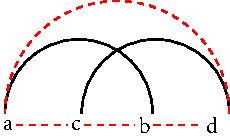
\includegraphics{figures/t_total_order}
    \caption[Book embedding constraints]{If $a < c < b < d$ occurs for two edges $\{a, b\}$ and $\{c,d\}$,
there is no page embedding with the order~$<$. Especially not a canonical one using semi-circles. The
red (dashed) edges result from adding the spine to the page embedding.}
    \label{figure:total}
\end{figure}

\noindent Since the pages in a book embedding problem are independent of each
other, we can use this lemma to rephrase the book embedding problem
as a total ordering problem.
\newProb{\probBookOrder}{A finite set $V := \range{n}$ and sets
$E_1,\dotsc, E_k \subseteq \binom{M}{2}$.}
{Is there a valid book order $<$ for all~$E_i$ where $i \in \range{k}$?}
\begin{theorem}
\label{lemma:all-book-constraints}
\probBook and \probBookOrder are equivalent.
\end{theorem}
\begin{myproof}
Follows by applying \myref{lemma:constraints} to each page.\qedhere
\end{myproof}

From this point onward, we use both representations of the book embedding problem
interchangeably. Whenever we refer to \probBook we also mean \probBookOrder and vice versa.
Note that the book constraints for two edges $\{a, b\}$ and $\{c, d\}$ are trivially fulfilled if
the edges have a common vertex. Therefore, we always assume that two edges are independent whenever
we check book constraints in the remainder of the thesis.

\section{Equivalent Orders}\label{section:symmetry}

We significantly reduced the number of basically equivalent ways to solve a book
embedding instance by restating the drawing problem \probBook as an ordering problem \probBookOrder. Still, several choices remain.
We determine some of them in this section, namely that the mirror image and any cyclic shift of a total order solving a \probBook instance still solve the instance. 

Notably, this knowledge proves useful for reducing other problems to book embedding in 
\myref{chapter:complexity} where we discuss the time complexity of \probBook.

By considering all mirror images and cyclic shifts of a total order to be the same
we turn the total order into what we call a \emph{symmetric order}.

\begin{figure}[\placement]\centering
    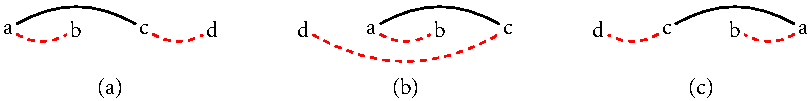
\includegraphics[width=\textwidth]{figures/t_symmetry}
    \caption[Equivalent orders]{A valid book embedding (a) with cyclic shift to the right by one element~(b)
and mirror image~(c).}
    \label{figure:symmetry}
\end{figure}

%\begin{definition}
Let~$M$ be an $n$-element set and~$O_M$ be the set of total orders (permutations) on~$M$.

For a permutation $\pi = (a_1, a_2, \dotsc, a_n) \in O_M$ we say that~$(a_n, a_{n-1}, \dotsc, a_1) \in O_M$ is the \emph{mirror image of~$\pi$} and~$(a_{n-k+1}, a_{n-k+2}, \dotsc, a_n, a_1, \dotsc, a_{n-k}) \in O_M$ is the \emph{cyclic shift of~$\pi$ by~$k$} for~$k \in \{0, \dotsc, n-1\}$. Both of these elementary operations are illustrated in \myref{figure:symmetry}.

We now define a relation~$\sim$ on~$O_M$. For all $a, b \in O_M$ we have
$a\sim b$ if and only if we can get~$b$ from~$a$ by a series of cyclic shifts
and mirror images. Clearly, the relation~$\sim$ is an equivalence relation.

Let~$\widetilde{O}_M$ be the set of equivalence classes of~$O_M$ with respect to~$\sim$. An
element~$o \in \widetilde{O}_M$ is then called a \emph{symmetric order on~$M$}. We write~$[\pi] := \{\tau \in O_M: \pi \sim \tau\} \in\widetilde{O}_M$ to refer to the symmetric order corresponding to a permutation~$\pi \in O_M$.
%A ternary relation~$[\cdot, \cdot, \cdot]$ on a set~$M$ is called a \emph{cyclic order} if the
%following constraints hold for all~$a, b, c, d \in M$:
%\begin{enumerate}
%\item If $[a, b, c]$, then~$[b, c, a]$. (\emph{cyclic})
%\item If $[a, b, c]$, then not $[c, b, a]$. (\emph{asymmetric}).
%\item If $[a, b, c]$ and $[a, c, d]$, then $[a, b, d]$. (\emph{transitive})
%\item If $a$, $b$ and $c$ are pairwise distinct, then either $[a, b, c]$ or
%$[c, b, a]$. (\emph{total})
%\end{enumerate}
%\end{definition}

Let~$<$ be a total order (permutation) on a finite set~$M$. We can order the elements
of~$M$ on a circle by starting at one point of the circle, going either clockwise
or counter-clockwise without making a full turn and writing the elements of~$M$ on distinct points in the order~$<$. 

Conversely, if we have an arrangement of a finite number of elements on distinct points of a circle, it is ambiguous which total order we got this arrangement from. We can cut the circle open between any two elements and get a total
order by going either clockwise or counter-clockwise. Clearly, the notion of a symmetric order is defined
exactly in such a manner that the orders we get from~$<$ (written on a circle) by cutting the circle open are the orders~$[<]$.

That is, a symmetric order can alternatively be interpreted as a way of ordering elements on a circle.
If we only consider cyclic shifts in the definition of~$\sim$, we get \emph{cyclic orders} which are
considered more often in the literature.
%It is unusual that we do not distinguish between the two directions (clockwise or counter-clockwise) of %the order, but we stick with this definition in this thesis.
%The natural interpretation of $[a, b, c]$ is: after~$a$, one
%reaches~$b$ before~$c$ on the cycle. Any linear order on~$M$ can be turned into a cyclic
%order by writing the elements of~$M$ from the smallest to the
%largest on a cycle. Similarly, we can get a linear order from a cyclic order
%by starting at any element and walking around the cycle in one direction.
%When turning a linear order~$<$ into a cyclic order and then transforming it into
%a linear order again, a different linear order may result. We call these orders \emph{cyclic rotations}
%of the original order~$<$. All of them can be constructed by a series of reflections and
%shifts to the right. Both of these elementary operations are illustrated in \myref{figure:symmetry}. We now show that any cyclic rotation of a valid book order remains valid.

We now show that cyclic shifts and mirror images preserve the validity of an order.

\begin{theorem}
\label{lemma:symmetry}
Let $(V, E_1),\dotsc, (V, E_k)$ be a book embedding instance with valid book order~$<\,\in O_V$.
Then any order $<_c\,\in [<]$ is valid.
\end{theorem}
\begin{myproof}
We show that the cyclic shift by one~$<_1$ of~$<$ and
the mirror image~$<_2$ of~$<$ are still valid orders. Then any order~$<_c\,\in [<]$ must also be valid.

To do so we show that a page~$(V, E_i)$ cannot have the forbidden substructure of \myref{lemma:constraints} in either order $<_1$ or~$<_2$.

If $a <_2 c <_2 < b <_2 d$ occurs for some~$\{a, b\}, \{c, d\} \in E_i$, we have $d < b < c < a \in E_i$ as $<_2$ is the reverse of~$<$, which
contradicts the validity of~$<$. Thus,~$<_2$ must be valid.

Similarly, assume the forbidden substructure $a <_1 c <_1 b <_1 d$ occurs for some~$\{a, b\}, \{c, d\} \in E_i$. If~$a$ is not the smallest element of~$V$ with respect to~$<_1$, we get~$a < c < b < d$ by construction of~$<_1$, a
contradiction to the validity of~$<$. Otherwise,
we get $c < b < d < a$, which again contradicts
the validity of~$<$. Thus,~$<_1$ is valid.
\end{myproof} 
 
%By applying an appropriate continuous
%deformation to it,  every page drawing is mapped to a planar drawing where all the
%vertices are on the unit circle and all edges lie inside of it.

%Reversely, there is a continuous deformation mapping the unit sphere
%to the upper half-plane and an arbitrary vertex on the cycle
%to the left-most vertex on the real line as well as traversing the cycle in an arbitrary
%direction. That is, we get a book embedding
%for all cyclic rotations of~$<$.
%%If we fix a book drawing with order $>$ and consider $\SR^2$
%%as the complex plane $\SC$, this is fairly clear:
%%Just apply the Mobius transformation $f$ which maps $\SR$ to the unit circle,
%%then the appropriate rotation around the origin and finally $f^{-1}$ to the drawing. This
%%yields a book drawing with the cyclic rotation as vertex order. Note that
%%the Mobius transformation~$f$ maps the half-planes bounded by $\SR$ to the half-planes
%%bounded by the unit circle, \ie the edges still lie in one of the half-planes bordered
%%by~$\SR$.
%\end{myproof}
%
%Since the validity of the order remains invariant under cyclic rotations, 
%the ordering problem for book embeddings is sometimes defined on cyclic
%orders. This is not significant, since a cyclic order can always be cut open at any vertex to 
%return to our setting of total orders. For this reason, we use cyclic orders and linear orders interchangeably in this thesis.
%%% Local Variables: 
%%% mode: latex
%%% TeX-master: "thesis"
%%% End: 
